% =====================================================================
% Wurzeldokument der Vorlage für Abschluss- und Seminararbeiten
% Übersetzen mit: pdflatex -> bibtex -> pdflatex -> pdflatex
% (Overleaf und latexmk erledigen das automatisch.)
% =====================================================================

% 'twoside=off' für die Onlineversion, 'twoside=on' für die Druckversion
\documentclass[12pt,twoside=off,listof=totoc,bibliography=totoc,appendixprefix,paper=a4,headings=small]{scrbook}

% Packages
% -----------------------------------
% Schrift und Sprache
\usepackage[T1]{fontenc}
\usepackage{lmodern}				% Schriftfamilie
\usepackage[ngerman]{babel}
\usepackage{csquotes}				% kontextabhängige Anführungszeichen (\enquote{...})
\usepackage{microtype}				% Mikrotypografie (besseres Schriftbild)
\setkomafont{disposition}{\bfseries}

% Seitenränder (bei Bedarf einkommentieren)
% \usepackage[
%   paper=a4paper,
%   left=12.5mm,
%   right=25mm,
%   top=25mm,
%   bottom=50mm,
%   bindingoffset=10mm]{geometry}	% Seitenränder und Bindungskorrektur

% Literaturverwaltung: apacite (Zitierstil APA) mit natbib-Befehlen
% (\citet, \citep, ...) und BibTeX. Bewusst kein biblatex/biber: biber ist
% deutlich langsamer und sprengt das Compile-Zeitlimit von Overleaf (Free).
% Nicht zusätzlich biblatex laden -- die Pakete sind inkompatibel.
\usepackage[natbibapa]{apacite}

% Grafiken
\usepackage{graphicx}				% Grafiken einfügen (pdf, png - jpg möglichst vermeiden)
\graphicspath{{./Bilder/}}			% Pfad zu den Bildern

% Tabellen
\usepackage{tabularx}
\usepackage{longtable}
\usepackage{ltablex}				% tabularx-Tabellen dürfen über Seiten umbrechen
\usepackage{multirow}
\usepackage{booktabs}				% schönere horizontale Linien (\toprule, \midrule, ...)

% Sonstiges
\usepackage{amsmath}				% mathematische Formeln
\usepackage{listings}				% Quellcode / Algorithmen
\lstset{
  basicstyle=\ttfamily\small,		% Schrift für Quellcode
  columns=fullflexible, keepspaces=true,	% normale Zeichenabstände, Einrückung bleibt erhalten
  numbers=left, numberstyle=\tiny,	% Zeilennummern
  frame=tb,							% Linie oberhalb und unterhalb
  captionpos=t,						% Beschriftung oberhalb (wie bei Tabellen)
  breaklines=true,					% lange Zeilen umbrechen
  showstringspaces=false
}
\usepackage{lscape}					% einzelne Seiten im Querformat
\usepackage{setspace}				% Zeilenabstand
% \usepackage{todonotes}			% ToDos im Dokument markieren

\newtheorem{mydef}{Merksatz}		% Merksätze und Beispiele mit fortlaufender Nummer
\newtheorem{bsp}{Beispiel}

% hyperref möglichst als letztes Paket laden
\usepackage[colorlinks,linkcolor=black,citecolor=black,urlcolor=black]{hyperref}

\hyphenation{voll-stän-di-gen}		% Worttrennungen global definieren

\setcounter{tocdepth}{1}			% Ebenen, die im Inhaltsverzeichnis angezeigt werden
\counterwithin{table}{chapter}
\counterwithin{figure}{chapter}

% Document
% -----------------------------------
\begin{document}

\frontmatter
    % Titelseite soll keine Kopf oder Fußzeile haben
\thispagestyle{empty}

% Alle Elemente sollen zentriert sein
\begin{center}

\vspace*{-10mm}

{\LARGE PROFESSUR FÜR \\WIRTSCHAFTSINFORMATIK\\[1mm]}
DER FREIEN UNIVERSITÄT BERLIN\\

\vspace*{1cm}


\includegraphics[width=0.18\textwidth]{fu_logo}

\vspace*{1cm}

% Art der Arbeit => (Bachelorarbeit, Masterarbeit, Seminararbeit)
{\Large \textbf{Abschlussarbeit}}\\ 

\vspace{1cm}

% Titel der Arbeit 
{\Large \textbf{Hier folgt der Titel}}\\ 
\vspace*{1mm}
{\Large \textbf{dieser kann auf bis zu drei}}\\ 
\vspace*{1mm}
{\Large \textbf{Zeilen verteilt werden, wenn nötig}}\\

\vspace{1.5cm}

% Name der verfassenden Person(en)
{\LARGE Vorname Nachname}\\[15mm]

% Begutachtung, Betreuung, Kontaktdaten und Abgabetermin
\parbox{120mm}{
\begin{large}
\begin{tabbing}
Begutachtung: \=Univ.-Prof. Dr. rer. pol. Natalia Kliewer\\
Betreuung: \>Vorname Nachname\\
Semester:\> Wintersemester 2026-2027\\
Verfasst von:\> Vorname Nachname\\ % alphabetische Reihenfolge (Nachname)
Matrikel-Nr.:\> 1234567\\
Adresse:\> Straße Nr, PLZ Ort\\
E-Mail:\> mail@mail.de\\
Telefon:\>030-123 456 78\\
Studienfach:\>Bachelor BWL\\[8mm]
\textbf{Abgabetermin:} \= \textbf{01. Januar 2099}\\
\end{tabbing}
\end{large}
}

\end{center}
\clearpage{\pagestyle{empty}\cleardoublepage}
				% Titelblatt
    \thispagestyle{empty}

\vspace*{1cm}

\begin{center}
    \textbf{Zusammenfassung}
\end{center}

\vspace*{1cm}

\noindent 
Das Abstract fasst die Arbeit in 150--250 Wörtern zusammen (bei einer Bachelorarbeit eher weniger, bei einer Masterarbeit eher mehr). Es sollte die Forschungslücke, die verwendete Methodik, die wichtigsten Ergebnisse und deren Implikationen beinhalten. Vermeiden Sie unnötige Details und konzentrieren Sie sich auf die Kernaussagen Ihrer Arbeit auf einer leicht verständlichen Flughöhe. Dieser füllende Blindtext zeigt zusammen mit den Anweisungen den ungefähren Umfang der deutschen Zusammenfassung. Lorem ipsum dolor sit amet, consectetuer adipiscing elit. Aenean commodo ligula eget dolor. Aenean massa. Cum sociis natoque penatibus et magnis dis parturient montes, nascetur ridiculus mus. Donec quam felis, ultricies nec, pellentesque eu, pretium quis, sem. Nulla consequat massa quis enim. Donec pede justo, fringilla vel, aliquet nec, vulputate eget, arcu. In enim justo, rhoncus ut, imperdiet a, venenatis vitae, justo. Nullam dictum felis eu pede mollis pretium. Integer tincidunt. Cras dapibus. Vivamus elementum semper nisi. Aenean vulputate eleifend tellus. Aenean leo ligula, ultricies nec, pellentesque eu, pretium quis, sem. Nulla consequat massa quis enim. Nullam dictum felis eu pede mollis pretium. Integer tincidunt. Cras dapibus. Vivamus elementum semper nisi. Aenean vulputate eleifend tellus. Aenean leo ligula, ultricies nec, pellentesque eu, pretium quis, sem. Nulla consequat massa quis enim. Nullam dictum felis eu pede mollis pretium. Integer tincidunt. Cras dapibus. Vivamus elementum semper nisi. Aenean vulputate eleifend tellus.

	% Abstract auf Deutsch
    \clearpage{\pagestyle{empty}\cleardoublepage}
    \thispagestyle{empty}


\vspace*{1cm}

\begin{center}
    \textbf{Abstract}
\end{center}

\vspace*{1cm}

\noindent 
The following placeholder text illustrates the abstract in English. Lorem ipsum dolor sit amet, consectetuer adipiscing elit. Aenean commodo ligula eget dolor. Aenean massa. Cum sociis natoque penatibus et magnis dis parturient montes, nascetur ridiculus mus. Donec quam felis, ultricies nec, pellentesque eu, pretium quis, sem. Nulla consequat massa quis enim. Donec pede justo, fringilla vel, aliquet nec, vulputate eget, arcu. In enim justo, rhoncus ut, imperdiet a, venenatis vitae, justo. Nullam dictum felis eu pede mollis pretium. Integer tincidunt. Cras dapibus. Vivamus elementum semper nisi. Aenean vulputate eleifend tellus. Aenean leo ligula, porttitor eu, consequat vitae, eleifend ac, enim. Aliquam lorem ante, dapibus in, viverra quis, feugiat a, tellus. Phasellus viverra nulla ut metus varius laoreet. Quisque rutrum. Aenean imperdiet. Etiam ultricies nisi vel augue. Curabitur ullamcorper ultricies nisi. Integer tincidunt. Cras dapibus. Vivamus elementum semper nisi. Aenean vulputate eleifend tellus. Aenean leo ligula, porttitor eu, consequat vitae, eleifend ac, enim. Aliquam lorem ante, dapibus in, viverra quis, feugiat a, tellus. Phasellus viverra nulla ut metus varius laoreet. Quisque rutrum. Aenean imperdiet. Etiam ultricies nisi vel augue. Curabitur ullamcorper ultricies nisi. Integer tincidunt. Cras dapibus. Vivamus elementum semper nisi. Aenean vulputate eleifend tellus. Aenean leo ligula, porttitor eu, consequat vitae, eleifend ac, enim. Aliquam lorem ante, dapibus in, viverra quis, feugiat a, tellus. Phasellus viverra nulla ut metus varius laoreet. Quisque rutrum. Aenean imperdiet. Etiam ultricies nisi vel augue. Curabitur ullamcorper ultricies nisi.	% Abstract auf Englisch
    \clearpage{\pagestyle{empty}\cleardoublepage}
    % Sperrvermerk: nur bei vertraulichen Unternehmensdaten einkommentieren
    % \thispagestyle{empty}


\vspace*{1cm}

\begin{center}
    \textbf{Sperrvermerk}
\end{center}

\vspace*{1cm}

\noindent 

Die vorgelegte (Bachelorarbeit, Masterarbeit) basiert auf internen, vertraulichen Daten und Informationen des Unternehmens ...... In diese Arbeit dürfen Dritte, mit Ausnahme der Gutachtenden und befugter Mitglieder des Prüfungsausschusses, ohne ausdrückliche Zustimmung des Unternehmens und der verfassenden Person keine Einsicht nehmen. Von diesem Verbot ausgenommen sind außerdem jene Personen, die auch ansonsten zur Einsichtnahme in die genannten Daten und Informationen befugt sind. Eine Vervielfältigung und Veröffentlichung der (Bachelorarbeit, Masterarbeit) ohne ausdrückliche Genehmigung – auch auszugsweise – ist nicht erlaubt.

\vspace{2cm}

\noindent
Berlin, den 01. Januar 2099

\vspace{3cm}

\hspace*{7cm}%
\dotfill\\
\hspace*{8.5cm}%
\textit{(Unterschrift)}
    % \clearpage{\pagestyle{empty}\cleardoublepage}

    \onehalfspacing						% Zeilenabstand ab hier 1,5-zeilig
    \tableofcontents					% Inhaltsverzeichnis
    \clearpage{\pagestyle{empty}\cleardoublepage}

    \listoffigures						% Abbildungsverzeichnis
    \clearpage{\pagestyle{empty}\cleardoublepage}

    \listoftables						% Tabellenverzeichnis
    \clearpage{\pagestyle{empty}\cleardoublepage}

    % Abkürzungsverzeichnis
% Abkürzungen alphabetisch sortiert eintragen. Jede Abkürzung wird bei der
% ersten Verwendung im Text ausgeschrieben, z. B. "Enterprise Resource
% Planning (ERP)", und danach nur noch abgekürzt verwendet.
% Allgemein übliche Abkürzungen (z. B., usw., vgl.) gehören nicht hinein.

\addchap{Abkürzungsverzeichnis}

\begin{tabular}{@{}p{3cm}l@{}}
API & Application Programming Interface \\
ERP & Enterprise Resource Planning \\
\end{tabular}
	% Abkürzungsverzeichnis
    \clearpage{\pagestyle{empty}\cleardoublepage}

% -----------------------------------
\mainmatter								% die einzelnen Kapitel
    \chapter{Einleitung}

Diese Vorlage dient als Grundlage für die formale und inhaltliche Gestaltung wissenschaftlicher Abschlussarbeiten an der Professur für Wirtschaftsinformatik der Freien Universität Berlin. Die Einleitung einer wissenschaftlichen Arbeit motiviert das Thema, grenzt den Untersuchungsgegenstand ab und macht die Relevanz der Forschungsfrage deutlich. Sie bereitet die Lesenden auf die nachfolgenden Kapitel vor und schafft ein klares Verständnis für Zielsetzung und Aufbau der Arbeit.
Hinweis zur Formatierung: Seitenzahlen, Seitenränder, Schrift und Überschriften sind in der \texttt{main.tex} bereits eingestellt und müssen nicht angepasst werden. Achten Sie darauf, dass keine Leerräume bzw. unmotivierten Leerzeilen in der Arbeit vorkommen.
Zwischen einer Kapitelüberschrift und der ersten Unterüberschrift sollte immer ein einleitender Text stehen, der in das Kapitel einführt und dessen Inhalt und Struktur kurz beschreibt. Vermeiden Sie es, direkt von einer Überschrift zur nächsten zu springen, ohne den Lesenden Orientierung zu geben.


\section{Problemumfeld}

Im Abschnitt \glqq{}Problemumfeld\grqq{} wird das wissenschaftliche oder praktische Problem beschrieben, das die Arbeit adressiert. Hier soll deutlich werden, warum das gewählte Thema relevant ist und in welchem Kontext es steht. Eine klare Einordnung in den Forschungsstand zeigt, welche Lücke die Arbeit schließt oder welche neue Perspektive sie eröffnet.
Die Darstellung sollte nachvollziehbar machen, worin die Herausforderung besteht und warum diese bearbeitet werden muss. Eine präzise Beschreibung des Problemumfelds bildet die Grundlage für eine klare Zielsetzung und Forschungsfrage.

In ac felis quis tortor malesuada pretium. Pellentesque auctor neque nec urna. Proin sapien ipsum, porta a, auctor quis, euismod ut, mi. Aenean viverra rhoncus pede. Pellentesque habitant morbi tristique senectus et netus et malesuada fames ac turpis egestas. Ut non enim eleifend felis pretium feugiat. Vivamus quis mi. Phasellus a est. Phasellus magna. In hac habitasse platea dictumst. Curabitur at lacus ac velit ornare lobortis. Curabitur a felis in nunc fringilla tristique. 

\section{Zielsetzung}

In diesem Abschnitt wird die Zielsetzung der Arbeit formuliert. Hier sollte präzise dargelegt werden, was die Arbeit erreichen soll: Welche Forschungsfrage wird beantwortet? Welche Hypothesen werden untersucht? Welche Erkenntnisse sollen gewonnen werden?
Die Zielsetzung sollte klar von der bloßen Themenbeschreibung abgegrenzt sein. Falls die Arbeit bewusst eingegrenzt wird – etwa auf bestimmte Methoden, Branchen oder theoretische Perspektiven – sollte diese Abgrenzung hier transparent gemacht werden. Eine präzise Zielsetzung erleichtert es den Lesenden, die nachfolgende Argumentation nachzuvollziehen und die Ergebnisse später einzuordnen.


\section{Aufbau der Arbeit}

Dieser Abschnitt gibt einen Überblick über die Struktur der Arbeit und beschreibt die Funktion der nachfolgenden Kapitel. Typischerweise umfasst eine wissenschaftliche Arbeit Kapitel zu Grundlagen, Methodik, Ergebnissen und Fazit.
Ein Musteraufbau könnte wie folgt aussehen: Nach der Einleitung werden in Kapitel 2 die theoretischen Grundlagen und der Stand der Forschung dargestellt. Kapitel 3 erläutert die verwendete Methodik. Kapitel 4 präsentiert die Ergebnisse der Untersuchung. Kapitel 5 fasst die Erkenntnisse zusammen, diskutiert die Grenzen der Arbeit und gibt einen Ausblick auf weiterführende Forschung.
Durch die frühzeitige Beschreibung der Argumentationslinie wird die Struktur der Arbeit transparent und für die Lesenden nachvollziehbar.



    \clearpage{\pagestyle{empty}\cleardoublepage}
    \chapter{Grundlagen des \glqq{}Themas\grqq{}}

Die \glqq{}inneren\grqq{} Kapitel (alle außer dem ersten und dem letzten) sollen spezifisch benannt werden. Generische Überschriften (Stand der Forschung, Problemstellung, Methodik usw.), die in jeder beliebigen Abschlussarbeit stehen könnten, sollen vermieden werden.
Das Kapitel \glqq{}Grundlagen\grqq{} legt die theoretische und begriffliche Basis für die gesamte Arbeit. Hier werden zentrale Konzepte definiert, der Stand der Forschung aufgearbeitet und theoretische Rahmenwerke vorgestellt. Eine saubere Begriffsarbeit ist essenziell: Fachbegriffe sollten bei ihrer ersten Verwendung erklärt und konsistent im gesamten Dokument verwendet werden.

\section{Umgang mit Abbildungen}

Abbildungen dienen dazu, komplexe Zusammenhänge visuell darzustellen und sollten nur dann eingefügt werden, wenn sie einen inhaltlichen Mehrwert bieten. Jede Abbildung muss im Text erläutert und referenziert werden (ein bloßes \glqq{}siehe Abbildung X\grqq{} reicht nicht). Nummerierung und Formatierung erfolgen automatisch -- eine Abbildung benötigt nur ein Label, das dann mit \verb|\ref{}| referenziert wird, wie hier bei Abbildung \ref{fig:bsp1}. Die Beschriftung (\verb|\caption|) steht bei Abbildungen unterhalb.

\begin{figure}[h]
	\centering
		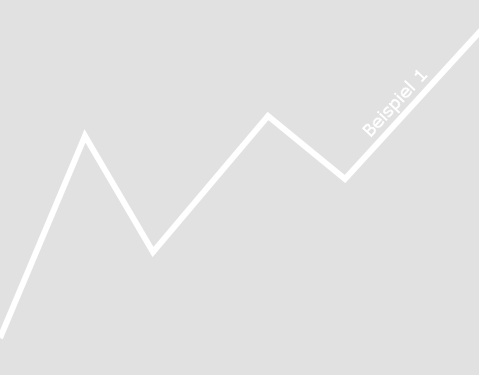
\includegraphics[width=0.4\textwidth]{./Bilder/bsp1.png}
	\caption{Beispiel 1 zum Einfügen einer Grafik}
	\label{fig:bsp1}
\end{figure}

\section{Umgang mit Tabellen}

Tabellen eignen sich zur strukturierten Darstellung von Daten, Vergleichen oder Übersichten. Wie bei Abbildungen gilt: Tabellen sollten nur eingefügt werden, wenn sie die Argumentation unterstützen und im Text erläutert werden. Ein Beispiel ist die Übersicht der Zitierbefehle in Tabelle \ref{tab:cite}. Die Beschriftung steht bei Tabellen oberhalb; für horizontale Linien werden \verb|\toprule|, \verb|\midrule| und \verb|\bottomrule| aus dem Paket \texttt{booktabs} verwendet, senkrechte Linien entfallen. Tabellen müssen Sie so gut wie nie von Hand abtippen:

\begin{itemize}
  \item \textbf{Tables Generator} (tablesgenerator.com) -- Excel-Bereich einfügen, LaTeX-Code exportieren.
  \item \textbf{Excel2LaTeX} -- Excel-Add-in, wandelt markierte Zellen per Knopfdruck um.
  \item \textbf{Generative KI} (ChatGPT, Claude \dots) wandelt eingefügte Tabellen zuverlässig um -- aber \textbf{jede Zahl danach gegen die Originaltabelle prüfen}, KI kann Werte vertauschen oder runden.
\end{itemize}

\section{Literaturverzeichnis}

Das Literaturverzeichnis listet alle in der Arbeit zitierten Quellen auf. Die Verwaltung erfolgt mit \texttt{BibTeX}; den Zitierstil APA liefert das Paket \texttt{apacite}, die Zitierbefehle stammen aus \texttt{natbib}. Verwenden Sie ein gängiges Zitierformat (z.\,B. APA, Harvard, IEEE) und wenden Sie dieses konsistent an. Nutzen Sie Literaturverwaltungssoftware wie Citavi, EndNote oder Zotero, um Ihre Referenzen als \texttt{.bib}-Datei zu exportieren, und speichern Sie diese als \texttt{Literatur/quellen.bib}; eingebunden wird sie am Ende von \texttt{main.tex} mit \verb|\bibliography{Literatur/quellen}|. Ins Literaturverzeichnis gelangen automatisch alle zitierten Quellen. Zum Übersetzen ist der Ablauf \texttt{pdflatex} $\rightarrow$ \texttt{bibtex} $\rightarrow$ \texttt{pdflatex} $\rightarrow$ \texttt{pdflatex} erforderlich; Overleaf erledigt das automatisch. Laden Sie nicht zusätzlich \texttt{biblatex}, da es mit \texttt{natbib} und \texttt{apacite} inkompatibel ist. \textbf{Abwandlungen} des Zitierbefehls werden in der Tabelle \ref{tab:cite} dargestellt und zeigen, wie das Zitat im Satz erscheint.

\begin{table}[htbp]
\centering
\footnotesize
\caption{Varianten der Zitierbefehle mit \texttt{natbib} und \texttt{apacite}}
\label{tab:cite}
\begin{tabular}{@{}ll@{}}
\toprule
\textbf{LaTeX-Quellcode} & \textbf{Ergebnis im PDF} \\
\midrule
\verb|\citep{kliewer2006time}| & \citep{kliewer2006time} \\
\verb|\citet{kliewer2006time}| & \citet{kliewer2006time} zeigen \dots \\
\verb|\citep[S.~1620]{kliewer2006time}| & \citep[S.~1620]{kliewer2006time} \\
\verb|\citep[vgl.][]{kliewer2006time}| & \citep[vgl.][]{kliewer2006time} \\
\verb|\citeauthor{kliewer2006time}| & \citeauthor{kliewer2006time} \\
\verb|\citeyear{kliewer2006time}| & \citeyear{kliewer2006time} \\
\verb|\citep{kliewer2006time,gopen1990science}| & \citep{kliewer2006time,gopen1990science} \\
\bottomrule
\end{tabular}
\end{table}

\noindent Die Faustregel: \textbf{\texttt{\textbackslash citep}} (\glqq{}parenthetical\grqq{}) setzt den \emph{gesamten} Verweis in Klammern und eignet sich, wenn die zitierten Personen nicht Teil des Satzes sind, z.\,B.: \glqq{}Die Nachfrage steigt bei höheren Temperaturen \citep{kliewer2006time}.\grqq{} \textbf{\texttt{\textbackslash citet}} (\glqq{}textual\grqq{}) macht die zitierten Personen grammatikalisch zum Satzsubjekt, z.\,B.: \glqq{}\citet{kliewer2006time} zeigen, dass \dots\grqq{} Über die optionalen Argumente in eckigen Klammern lassen sich Seitenangaben oder Zusätze wie \glqq{}vgl.\grqq{} ergänzen.

\section{Formatierung}

Die gesamte Arbeit sollte einheitlich formatiert sein. In Word pflegt man dafür Formatvorlagen manuell; in LaTeX sind alle Einstellungen (Schrift, Seitenränder, Zeilenabstand, Seitenzahlen, Überschriften und Verzeichnisse) zentral in der \texttt{main.tex} getroffen und müssen nicht angepasst werden. Werden zusätzliche Funktionen benötigt, können dort weitere Pakete ergänzt werden.

    \clearpage{\pagestyle{empty}\cleardoublepage}
    \chapter{"`Eigenanteil"': Konzept, Analyse, Experiment etc.}

In diesem Kapitel steht der Eigenanteil der Arbeit. Je nach Thema ist das zum Beispiel die konzeptionelle Darstellung der gewählten Methode, die Aufbereitung von Erkenntnissen aus der Literatur oder die Synthese mehrerer Erkenntnisse zu einem eigenen Ansatz, Modell oder Experiment. Wie alle inneren Kapitel sollte auch dieses Kapitel spezifisch benannt werden. Ein mehrstufiges Vorgehen, etwa Konzept, Umsetzung und Evaluation, kann auch auf mehrere Kapitel aufgeteilt werden.

\section{Erster Abschnitt}

 Etiam sit amet orci eget eros faucibus tincidunt. Duis leo. Sed fringilla mauris sit amet nibh. Donec sodales sagittis magna. Sed consequat, leo eget bibendum sodales, augue velit cursus nunc, quis gravida magna mi a libero. Fusce vulputate eleifend sapien. Vestibulum purus quam, scelerisque ut, mollis sed, nonummy id, metus. Nullam accumsan lorem in dui. Cras ultricies mi eu turpis hendrerit fringilla. Vestibulum ante ipsum primis in faucibus orci luctus et ultrices posuere cubilia Curae; In ac dui quis mi consectetuer lacinia. Nam pretium turpis et arcu. Duis arcu tortor, suscipit eget, imperdiet nec, imperdiet iaculis, ipsum. Sed aliquam ultrices mauris. Integer ante arcu, accumsan a, consectetuer eget, posuere ut, mauris. Praesent adipiscing. Phasellus ullamcorper ipsum rutrum nunc. Nunc nonummy metus. Vestibulum volutpat pretium libero. Cras id dui. Aenean ut eros et nisl sagittis vestibulum. Nullam nulla eros, ultricies sit amet, nonummy id, imperdiet feugiat, pede. Sed lectus. Donec mollis hendrerit risus. Phasellus nec sem in justo pellentesque facilisis. Etiam imperdiet imperdiet orci. Nunc nec neque. Phasellus leo dolor, tempus non, auctor et, hendrerit quis, nisi. Curabitur ligula sapien, tincidunt non, euismod vitae, posuere imperdiet, leo. Maecenas malesuada. 
\begin{figure}
	\centering
		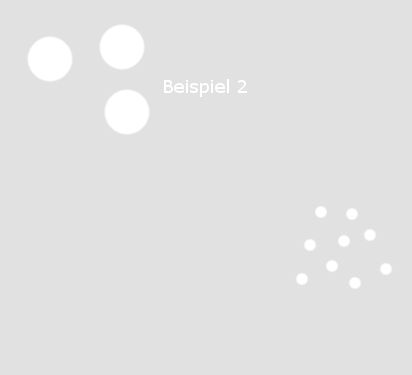
\includegraphics{./Bilder/bsp2.png}
	\caption{Beispiel 2 zum Einfügen einer Grafik}
	\label{fig:bsp2}
\end{figure}
 
Praesent congue erat at massa. Sed cursus turpis vitae tortor. Donec posuere vulputate arcu. Phasellus accumsan cursus velit. Vestibulum ante ipsum primis in faucibus orci luctus et ultrices posuere cubilia Curae; Sed aliquam, nisi quis porttitor congue, elit erat euismod orci, ac placerat dolor lectus quis orci. Phasellus consectetuer vestibulum elit. Aenean tellus metus, bibendum sed, posuere ac, mattis non, nunc. Vestibulum fringilla pede sit amet augue. In turpis. Pellentesque posuere. Praesent turpis. Aenean posuere, tortor sed cursus feugiat, nunc augue blandit nunc, eu sollicitudin urna dolor sagittis lacus. Donec elit libero, sodales nec, volutpat a, suscipit non, turpis. Nullam sagittis. Suspendisse pulvinar, augue ac venenatis condimentum, sem libero volutpat nibh, nec pellentesque velit pede quis nunc. Vestibulum ante ipsum primis in faucibus orci luctus et ultrices posuere cubilia Curae; Fusce id purus. Ut varius tincidunt libero. Phasellus dolor. 
 
\begin{table}[htbp]
	\centering
	\caption{Beispiel zum Einfügen einer Tabelle}
	\label{tab:Betreuungsende}
	\begin{tabular}{lrl}
		\toprule
		\textbf{Taxonomie} & \textbf{Anzahl} & \textbf{Rohdatenwerte} \\
		\midrule
		Verstorben & 104 & (verstorben) \\
		Pflegeheim & 88  & (geht in stationäre Einrichtung), (ist im Heim), \dots \\
		Genesen    & 77  & (genesen), (Wunde abgeheilt), (Wunde verheilt) \\
		\bottomrule
	\end{tabular}
\end{table}

Maecenas vestibulum mollis diam. Pellentesque ut neque. Pellentesque habitant morbi tristique senectus et netus et malesuada fames ac turpis egestas. In dui magna, posuere eget, vestibulum et, tempor auctor, justo. In ac felis quis tortor malesuada pretium. Pellentesque auctor neque nec urna. Proin sapien ipsum, porta a, auctor quis, euismod ut, mi. Aenean viverra rhoncus pede. Pellentesque habitant morbi tristique senectus et netus et malesuada fames ac turpis egestas. Ut non enim eleifend felis pretium feugiat. Vivamus quis mi. Phasellus a est. Phasellus magna. In hac habitasse platea dictumst. Curabitur at lacus ac velit ornare lobortis. Curabitur a felis in nunc fringilla tristique. Lorem ipsum dolor sit amet, consectetuer adipiscing elit. Aenean commodo ligula eget dolor. Aenean massa. Cum sociis natoque penatibus et magnis dis parturient montes, nascetur ridiculus mus. Donec quam felis, ultricies nec, pellentesque eu, pretium quis, sem. Nulla consequat massa quis enim. Donec pede justo, fringilla vel, aliquet nec, vulputate eget, arcu. In enim justo, rhoncus ut, imperdiet a, venenatis vitae, justo. Nullam dictum felis eu pede mollis pretium. Integer tincidunt. Cras dapibus. Vivamus elementum semper nisi. Aenean vulputate eleifend tellus. Aenean leo ligula, porttitor eu, consequat vitae, eleifend ac, enim. Aliquam lorem ante, dapibus in, viverra quis, feugiat a, tellus. Phasellus viverra nulla ut metus varius laoreet. Quisque rutrum. Aenean imperdiet. Etiam ultricies nisi vel augue. Curabitur ullamcorper ultricies nisi. Nam eget dui. Etiam rhoncus (...)

\section{Zweiter Abschnitt}

Maecenas tempus, tellus eget condimentum rhoncus, sem quam semper libero, sit amet adipiscing sem neque sed ipsum. Nam quam nunc, blandit vel, luctus pulvinar, hendrerit id, lorem. Maecenas nec odio et ante tincidunt tempus. Donec vitae sapien ut libero venenatis faucibus. Nullam quis ante. Etiam sit amet orci eget eros faucibus tincidunt. Duis leo. Sed fringilla mauris sit amet nibh. Donec sodales sagittis magna. Sed consequat, leo eget bibendum sodales, augue velit cursus nunc, quis gravida magna mi a libero. Fusce vulputate eleifend sapien. Vestibulum purus quam, scelerisque ut, mollis sed, nonummy id, metus. Nullam accumsan lorem in dui. Cras ultricies mi eu turpis hendrerit fringilla. Vestibulum ante ipsum primis in faucibus orci luctus et ultrices posuere cubilia Curae; In ac dui quis mi consectetuer lacinia. Nam pretium turpis et arcu. Duis arcu tortor, suscipit eget, imperdiet nec, imperdiet iaculis, ipsum. Sed aliquam ultrices mauris. Integer ante arcu, accumsan a, consectetuer eget, posuere ut, mauris. Praesent adipiscing. Phasellus ullamcorper ipsum rutrum nunc. Nunc nonummy metus. Vestibulum volutpat pretium libero. Cras id dui. Aenean ut eros et nisl sagittis vestibulum. Nullam nulla eros, ultricies sit amet, nonummy id, imperdiet feugiat, pede. Sed lectus. Donec mollis hendrerit risus. Phasellus nec sem in justo pellentesque facilisis. Etiam imperdiet imperdiet orci. Nunc nec neque. Phasellus leo dolor, tempus non, auctor et, hendrerit quis, nisi. Curabitur ligula sapien, tincidunt non, euismod vitae, posuere imperdiet, leo. Maecenas malesuada. Praesent congue erat at massa. Sed cursus turpis vitae tortor. Donec posuere vulputate arcu. Phasellus accumsan cursus velit. Vestibulum ante ipsum primis in faucibus orci luctus et ultrices posuere cubilia Curae; Sed aliquam, nisi quis porttitor congue, elit erat euismod orci, ac placerat dolor lectus quis orci. Phasellus consectetuer vestibulum elit. Aenean tellus metus, bibendum sed, posuere ac, mattis non, nunc. Vestibulum fringilla pede sit amet augue. In turpis. Pellentesque posuere. Praesent turpis. Aenean posuere, tortor sed cursus feugiat, nunc augue blandit nunc, eu sollicitudin urna dolor sagittis lacus. Donec elit libero, sodales nec, volutpat a, suscipit non, turpis. Nullam sagittis. Suspendisse pulvinar, augue ac venenatis condimentum, sem libero volutpat nibh, nec pellentesque velit pede quis nunc. Vestibulum ante ipsum primis in faucibus orci luctus et ultrices posuere cubilia Curae; Fusce id purus. Ut varius tincidunt libero. Phasellus dolor. Maecenas vestibulum mollis diam. Pellentesque ut neque. Pellentesque habitant morbi tristique senectus et netus et malesuada fames ac turpis egestas. In dui magna, posuere eget, vestibulum et, tempor auctor, justo. In ac felis quis tortor malesuada pretium. Pellentesque auctor neque nec urna. Proin sapien ipsum, porta a, auctor quis, euismod ut, mi. Aenean viverra rhoncus pede. Pellentesque habitant morbi tristique senectus et netus et malesuada fames ac turpis egestas. Ut non enim eleifend felis pretium feugiat. Vivamus quis mi. Phasellus a est. Phasellus magna. In hac habitasse platea dictumst. Curabitur at lacus ac velit ornare lobortis. Curabitur a felis in nunc fringilla tristique. Lorem ipsum dolor sit amet, consectetuer adipiscing elit. Aenean commodo ligula eget dolor. Aenean massa. Cum sociis natoque penatibus et magnis dis parturient montes, nascetur ridiculus mus. Donec quam felis, ultricies nec, pellentesque eu, pretium quis, sem. Nulla consequat massa quis enim. Donec pede justo, fringilla vel, aliquet nec, vulputate eget, arcu. In enim justo, rhoncus ut, imperdiet a, venenatis vitae, justo. Nullam dictum felis eu pede mollis pretium. Integer tincidunt. Cras dapibus. Vivamus elementum semper nisi. Aenean vulputate eleifend tellus. Aenean leo ligula, porttitor eu, consequat vitae, eleifend ac, enim. Aliquam lorem ante, dapibus in, viverra quis, feugiat a, tellus. Phasellus viverra nulla ut metus varius laoreet. Quisque rutrum. Aenean imperdiet. Etiam ultricies nisi vel augue. Curabitur ullamcorper ultricies nisi. Nam eget dui. Etiam rhoncus. Maecenas tempus, tellus eget condimentum rhoncus, sem quam semper libero, sit amet adipiscing sem neque sed ipsum. Nam quam nunc, blandit vel, luctus pulvinar, hendrerit id, lorem. Maecenas nec odio et ante tincidunt tempus. Donec vitae sapien ut libero venenatis faucibus. Nullam quis ante. Etiam sit amet orci eget eros faucibus tincidunt. Duis leo. Sed fringilla mauris sit amet nibh. Donec sodales sagittis magna. Sed consequat, leo eget bibendum sodales, augue velit cursus nunc, quis gravida magna mi a libero. Fusce vulputate eleifend sapien. Vestibulum purus quam, scelerisque ut, mollis sed, nonummy id, metus. Nullam accumsan lorem in dui. Cras ultricies mi eu turpis hendrerit fringilla. Vestibulum ante ipsum primis in faucibus orci luctus et ultrices posuere cubilia Curae; In ac dui quis mi consectetuer lacinia. Nam pretium turpis et arcu. Duis arcu tortor, suscipit eget, imperdiet nec, imperdiet iaculis, ipsum. Sed aliquam ultrices mauris. Integer ante arcu, accumsan a, consectetuer eget, posuere ut, mauris. Praesent adipiscing. Phasellus ullamcorper ipsum rutrum nunc. Nunc nonummy metus. Vestibulum volutpat pretium libero. Cras id dui. Aenean ut eros et nisl sagittis vestibulum. Nullam nulla eros, ultricies sit amet, nonummy id, imperdiet feugiat, pede. Sed lectus. Donec mollis hendrerit risus. Phasellus nec sem in justo pellentesque facilisis. Etiam imperdiet imperdiet orci. Nunc nec neque. Phasellus leo dolor, tempus non, auctor et, hendrerit quis, nisi. Curabitur ligula sapien, tincidunt non, euismod vitae, posuere imperdiet, leo. Maecenas malesuada. Praesent congue erat at massa. Sed cursus turpis vitae tortor. Donec posuere vulputate arcu. Phasellus accumsan cursus velit. Vestibulum ante ipsum primis in faucibus orci luctus et ultrices posuere cubilia Curae; Sed aliquam, nisi quis porttitor congue, elit erat euismod orci, ac placerat dolor lectus quis orci. Phasellus consectetuer vestibulum elit. Aenean tellus metus, bibendum sed, posuere ac, mattis non, nunc. Vestibulum fringilla pede sit amet augue. In turpis. Pellentesque posuere. Praesent turpis. Aenean posuere, tortor sed cursus feugiat, nunc augue blandit nunc, eu sollicitudin urna dolor sagittis lacus. Donec elit libero, sodales nec, volutpat a, suscipit non, turpis.


\section{Formeln}

Abgesetzte Formeln werden in der Umgebung \verb|equation| gesetzt und automatisch nummeriert. Im Text wird mit \verb|\eqref{}| auf sie verwiesen, etwa auf den arithmetischen Mittelwert in Gleichung \eqref{eq:mittelwert}:
\begin{equation}
	\bar{x} = \frac{1}{n} \sum_{i=1}^{n} x_i
	\label{eq:mittelwert}
\end{equation}
Alle Symbole werden direkt im Anschluss erklärt: Dabei bezeichnet $n$ die Anzahl der Beobachtungen und $x_i$ den $i$-ten Messwert. Kurze Formeln innerhalb eines Satzes stehen zwischen Dollarzeichen, z.\,B. \verb|$a^2 + b^2 = c^2$| für $a^2 + b^2 = c^2$. Mehrzeilige Formeln lassen sich mit der Umgebung \verb|align| aus dem Paket \texttt{amsmath} untereinander ausrichten.

\section{Quellcode}

Kurze Quellcode-Ausschnitte werden mit der Umgebung \verb|lstlisting| aus dem Paket \texttt{listings} eingebunden und wie Abbildungen mit Beschriftung und Label versehen (siehe Listing \ref{lst:mittelwert}). Längere Programme gehören in den Anhang oder in ein Repository\footnote{Zum Beispiel GitHub oder GitLab. Der Link wird dann, wie hier gezeigt, in einer Fußnote angegeben.}; eine ganze Datei lässt sich mit \verb|\lstinputlisting{Pfad/zur/Datei}| einbinden. Die Programmiersprache wird über die Option \verb|language| angegeben, damit Schlüsselwörter hervorgehoben werden.

\begin{lstlisting}[language=Python, caption={Berechnung des arithmetischen Mittelwerts}, label={lst:mittelwert}]
# Berechnet den arithmetischen Mittelwert einer Liste
def mittelwert(werte):
    return sum(werte) / len(werte)

print(mittelwert([2, 4, 9]))  # Ausgabe: 5.0
\end{lstlisting}

\section{Weitere Abschnitte (...)}

Nullam sagittis (...) 
    \clearpage{\pagestyle{empty}\cleardoublepage}
    \chapter{Ergebnisse}

Zwischen einer Kapitelüberschrift und der ersten Unterüberschrift sollte immer ein einleitender Text stehen, der in das Kapitel einführt und dessen Inhalt und Struktur kurz beschreibt. Vermeiden Sie es, direkt von einer Überschrift zur nächsten zu springen, ohne den Lesenden Orientierung zu geben.

\section{Erster Abschnitt}
Im Kapitel \glqq{}Ergebnisse\grqq{} werden die Befunde der Untersuchung sachlich, nachvollziehbar und strukturiert dargestellt. Die Darstellung sollte sich an der Forschungsfrage oder der gewählten Methodik orientieren. Ziel ist es, die Lesenden in die Lage zu versetzen, die Ergebnisse zu verstehen und nachzuvollziehen, ohne dass bereits eine umfassende Interpretation oder Diskussion erfolgt.
Hinweise zur Darstellung:
\begin{itemize}
    \item \textbf{Strukturierung}: Gliedern Sie die Ergebnisse logisch, etwa nach Forschungsfragen, Hypothesen oder methodischen Schritten.
    \item \textbf{Objektivität}: Vermeiden Sie wertende Aussagen. Interpretationen gehören in die Diskussion oder das Fazit.
    \item \textbf{Visualisierung}: Nutzen Sie Tabellen, Abbildungen oder Diagramme, um komplexe Ergebnisse verständlich darzustellen. Jede Visualisierung muss im Text erläutert werden.
    \item \textbf{Nachvollziehbarkeit}: Beschreiben Sie die Ergebnisse so, dass die Lesenden die Schlussfolgerungen nachvollziehen können, ohne die Rohdaten einsehen zu müssen.
\end{itemize}
Falls die Arbeit eine klare Trennung zwischen Ergebnisdarstellung und Interpretation vorsieht, sollte diese hier eingehalten werden. In manchen Fachbereichen werden Ergebnisse und Diskussion getrennt, in anderen gemeinsam behandelt. Orientieren Sie sich an den fachspezifischen Konventionen und den Vorgaben Ihrer Betreuung.
    \clearpage{\pagestyle{empty}\cleardoublepage}
    \chapter{Fazit und Ausblick}

Das letzte Kapitel schließt die Arbeit ab. Es fasst die wesentlichen Ergebnisse knapp zusammen und beantwortet die in der Einleitung gestellte Forschungsfrage ausdrücklich. Neue Ergebnisse oder Quellen werden hier nicht mehr eingeführt.

Typische Bestandteile sind:
\begin{itemize}
    \item \textbf{Fazit}: Zusammenfassung der zentralen Erkenntnisse und Antwort auf die Forschungsfrage.
    \item \textbf{Implikationen}: Bedeutung der Ergebnisse für Forschung und Praxis.
    \item \textbf{Limitationen}: Grenzen der eigenen Arbeit, etwa durch Datenbasis, Methode oder Annahmen, und deren Einfluss auf die Aussagekraft der Ergebnisse.
    \item \textbf{Ausblick}: offene Fragen und mögliche Ansatzpunkte für weiterführende Forschung.
\end{itemize}
Je nach Umfang können diese Punkte in eigenen Unterkapiteln behandelt werden.

    \clearpage{\pagestyle{empty}\cleardoublepage}
    \appendix
    \chapter{Appendix}

\begin{table}[htbp]
  \centering
  \footnotesize
  \caption{Beispiel Anhang Tabelle 1}
  \label{tab:addlabel}
    \begin{tabular}{@{}lllll@{}}
    \toprule
    \textbf{Name} & \textbf{URL} & \textbf{OC-Typ} & \textbf{Modell} & \textbf{Gründungsjahr} \\
    \midrule
    Solavei & http://www.solavei.com & I.-o. & S.-M. & 2011 \\
    Spreaker & http://www.spreaker.com & I.-o. & S.-M. & 2009 \\
    Spreecast & http://www.spreecast.com & R.-o. & A.-M. &  \\
    Spring.me & http://www.spring.me & R.-o. & A.-M. & 2013 \\
    Sqeeqee & http://sqeeqee.com & R.-o. & A.-M. & 2012 \\
    Sulia & http://sulia.com & I.-o. & A.-M. & 2009 \\
    Tagged & http://www.tagged.com & R.-o. & A.-M. & 2004 \\
    Thinglink & http://www.thinglink.com & I.-o. & S.-M. & 2010 \\
    ThisNext & http://www.thisnext.com & I.-o. & T.-M. & 2005 \\
    Topic & http://trytopic.com & I.-o. & T.-M. &  \\
    Upfront Media Group & http://beupfront.com & R.-o. & S.-M. & 2012 \\
    Upworthy & http://www.upworthy.com & I.-o. & A.-M. & 2012 \\
    UrbanSitter & http://www.urbansitter.com & I.-o. & S.-M. & 2010 \\
    VoteIt & http://www.voteit.com & I.-o. & S.-M. & 2011 \\
    We Heart It & http://weheartit.com & I.-o. & A.-M. & 2007 \\
    Webtalk & http://webtalk.org & R.-o. & A.-M. & 2010 \\
    WeWork & http://www.wework.com & I.-o. & S.-M. & 2010 \\
    Written & http://written.com & I.-o. & T.-M. &  \\
    YeHive & http://www.yehive.com & R.-o. & A.-M. & 2012 \\
    Zao.com & http://www.zao.com & I.-o. & T.-M. & 2011 \\
    Facebook & http://facebook.com & R.-o. & A.-M. & 2004 \\
    LinkedIn & http://linkedin.com & R.-o. & S.-M. & 2003 \\
    Zoosk & http://www.zoosk.com & I.-o. & S.-M. & 2007 \\
    \bottomrule
    \end{tabular}
\end{table}

    \clearpage{\pagestyle{empty}\cleardoublepage}

% -----------------------------------
\backmatter
\bibliographystyle{apacite}			% Literaturverzeichnis im APA-Stil
\bibliography{Literatur/quellen}		% Pfad zur .bib-Datei (ohne Endung)
\clearpage{\pagestyle{empty}\cleardoublepage}
\markboth{}{}
\newpage
\thispagestyle{empty}
\noindent
\section*{Eigenständigkeitserklärung}
1. Hiermit versichere ich,
\begin{itemize}
    \item dass ich die von mir vorgelegte Arbeit selbständig abgefasst habe,
    \item dass ich keine weiteren Hilfsmittel verwendet habe als diejenigen, die im Vorfeld explizit zugelassen und von mir angegeben wurden,
    \item dass ich die Stellen der Arbeit, die dem Wortlaut oder dem Sinn nach anderen Werken (dazu zählen auch Internetquellen und KI-basierte Tools) entnommen sind, unter Angabe der Quelle kenntlich gemacht habe und
    \item dass ich die vorliegende Arbeit noch nicht für andere Prüfungen eingereicht habe.
\end{itemize}
2. Mir ist bewusst,
\begin{itemize}
    \item dass ich diese Prüfung nicht bestanden habe, wenn ich die mir bekannte Frist für die Einreichung meiner schriftlichen Arbeit versäume,
    \item dass ich im Falle eines Täuschungsversuchs diese Prüfung nicht bestanden habe,
    \item dass ich im Falle eines schwerwiegenden Täuschungsversuchs ggf. die Gesamtprüfung endgültig nicht bestanden habe und in diesem Studiengang nicht mehr weiter studieren darf und
    \item dass ich, sofern ich zur Erstellung dieser Arbeit KI-basierter Tools verwendet habe, die Verantwortung für eventuell durch die KI generierte fehlerhafte oder verzerrte (bias) Inhalte, fehlerhafte Referenzen, Verstöße gegen das Datenschutz- und Urheberrecht oder Plagiate trage.
\end{itemize}

\vspace{1cm}

\noindent
Berlin, den \today

\vspace{1cm}

\hspace*{7cm}%
\dotfill\\
\hspace*{8.5cm}%
\textit{(Unterschrift)}

\clearpage{\pagestyle{empty}\cleardoublepage}
% Tabellen-Einstellungen für dieses Formular (tabularx-Tabellen werden durch
% ltablex zu longtables und können über Seiten umbrechen)
\keepXColumns
\renewcommand{\theHtable}{ki.\arabic{table}} % eindeutige Hyperref-Anker (sonst Konflikt mit Tabelle A.1)
\setlength{\extrarowheight}{2pt}
\newcolumntype{L}{>{\raggedright\arraybackslash}X}

% --------------------------------------------------
% Erklärung zur Nutzung von generativen KI-Tools
% --------------------------------------------------

\section*{Erklärung zur Nutzung von generativen KI-Tools in Hochschulprüfungen}

\noindent
(In Anlehnung an \citealp{gimpel2023kognition})\\[0.5\baselineskip]
Die Erklärung soll für Seminar-, Projekt-, Bachelor- und Masterarbeiten verwendet werden, um die Nutzung von generativen KI-Tools und die eigene wissenschaftliche Leistung zu erläutern.

\vspace{1em}

\noindent
\textbf{Titel der Arbeit} \rule{0.7\textwidth}{0.4pt}\\[0.6\baselineskip]
\textbf{Abgabedatum} \rule{0.7\textwidth}{0.4pt}

\vspace{2em}

\subsection*{1. Verantwortungsvoller Umgang mit KI-Tools}

Bestätigen Sie die folgenden Aussagen.
\begingroup
\small
\begin{tabularx}{\textwidth}{|L|L|}
\hline
\textbf{Aussagen zum verantwortungsvollen Umgang mit KI-Tools} &
\textbf{Bestätigung: Ja} \\
\hline
Ich bin/wir sind über die Möglichkeiten und Grenzen der von mir/uns
verwendeten generativen KI-Tools informiert. &
 \\
\hline
Ich/wir habe(n) mich/uns vergewissert, dass die von den KI-Tools
gelieferten Ergebnisse korrekt sind, oder dass ich/wir sie korrigiert
habe(n). &
 \\
\hline
Ich/wir erkenne(n) an, dass die Verantwortung für die Arbeit bei
den Verfassenden liegt, nicht bei den KI-Tools oder einer anderen
Person. &
 \\
\hline
\end{tabularx}
\endgroup


\subsection*{2. Detaillierte Tätigkeiten, für die KI-Tools genutzt wurden}
Geben Sie an, welches KI-Tool Sie in welchem Umfang für welche Tätigkeit genutzt haben.
\begingroup
\small

\begin{tabularx}{\textwidth}{|L|L|L|L|}
\hline
\textbf{Aktivität} &
\textbf{Beschreibung} &
\textbf{Verwendete KI-Tools}\textsuperscript{*} \newline \scriptsize (falls zutreffend) &
\textbf{Beschreibung der Nutzung der KI-Tools} \newline \scriptsize (Art der Nutzung, betroffene Abschnitte der Arbeit, etc.) \\
\hline
\endhead
\hline
\endfoot
\textbf{Ideenfindung \& Konzeptualisierung} &
– Entwicklung von Ideen, Forschungszielen, Zielsetzungen und Forschungsfragen \newline
– Identifikation und Definition relevanter Konzepte &
&
\\
\hline
\textbf{Literaturrecherche und -analyse} &
– Suche nach relevanter Literatur \newline
– Überprüfung von potenziell relevanter Literatur \newline
– Zusammenfassungen von relevanter Literatur &
&
\\
\hline
\textbf{Methodik} &
– Suche nach einer geeigneten Methodik \newline
– Entwicklung und Anpassung der Methodik an die Forschungsfrage(n) &
&
\\
\hline
\textbf{Coding} &
– Erstellen und Dokumentieren von Code, Algorithmen, Software \newline
– Testen und Debuggen von bestehendem Code, Algorithmen, Software \newline
– Verständnis von bestehendem Code, Algorithmen, Software &
&
\\
\hline
\textbf{Datenerhebung und -analyse} &
– Erhebung von Primär- oder Sekundärdaten \newline
– Qualitative Datenanalyse (einschließlich Zusammenfassungen und Coding) \newline
– Quantitative Datenanalyse (einschließlich statistische Auswertung) \newline
– Mathematische, computergestützte oder andere formale Techniken zur Modellierung, Simulation und Analyse &
&
\\
\hline
\textbf{Interpretation und Validierung} &
– Interpretation der Ergebnisse \newline
– Ableitung von Implikationen für Forschung und Praxis \newline
– Überprüfung der allgemeinen Replikation/Reproduzierbarkeit der Ergebnisse und anderer Forschungsergebnisse &
&
\\
\hline
\textbf{Strukturierung und Planung des Textes} &
– Gliederung der Arbeit \newline
– Gliederung von Abschnitten der Arbeit (z.\,B. Stichpunktliste pro Abschnitt) &
&
\\
\hline

\textbf{Generierung des Textes} &
– Generierung von Text zu verschiedenen Themen in verschiedenen Abschnitten der Arbeit (einschließlich Titel und Zusammenfassungen) &
&
\\
\hline
\textbf{Übersetzen von Text} &
– Übersetzung selbst verfasster Texte \newline
– Übersetzung von anderen verfasster Texte &
&
\\
\hline
\textbf{Überprüfung \& Editierung des Textes} &
– Kritische Überprüfung, Feedback oder Überarbeitung des Inhalts, der Organisation oder der Grammatik der Arbeit \newline
– Korrekturlesen \newline
– Umformulierung oder Paraphrasierung von Text \newline
– Kürzung/Erweiterung des Textes &
&
\\
\hline
\textbf{Präsentation} &
– Strukturierung einer Präsentation über die Arbeit \newline
– Füllen einer Präsentation über die Arbeit mit Inhalt &
&
\\
\hline
\textbf{Quellenverwaltung} &
– Erstellen der Referenzliste \newline
– Formatierung der Referenzen &
&
\\
\hline
\textbf{Weitere Aktivitäten} & & & \\
\end{tabularx}
\endgroup
\vspace{2em}
\noindent\scriptsize
\textsuperscript{*}\,In Spalte 3 (Verwendete KI-Tools) nennen Sie bitte die konkrete Bezeichnung und Version der eingesetzten Tools (z.\,B. ChatGPT (Version xx), Perplexity, DeepL Write usw.). In Spalte 4 (Beschreibung der Nutzung) beschreiben Sie knapp, wie das Tool eingesetzt wurde (Art der Nutzung) und auf welche Teile der Arbeit sich die Nutzung bezog (z.\,B. „Überarbeitung der Diskussion“, „Entwurf der Gliederung“, „erste Textfassung des Abschnitts 3.2“).
\vspace{2em}

\subsection*{3. Ergänzende Angaben}

Gibt es sonst noch etwas, das Sie bezüglich der Nutzung von KI-Tools angeben wollen, welches Ihre eigenständige, definierbare Leistung bei der Erstellung dieser Arbeit hervorheben oder einschränken würde?

\vspace{1\baselineskip}
\noindent\rule{\textwidth}{0.4pt}\\[0.8\baselineskip]
\noindent\rule{\textwidth}{0.4pt}\\[0.8\baselineskip]
\noindent\rule{\textwidth}{0.4pt}

\vspace{2em}

\subsection*{4. Unterschrift(en) der Verfassenden}

\begingroup
\small

\begin{tabularx}{\textwidth}{|X|X|X|X|}
\hline
\textbf{Name} &
\textbf{Immatrikulations Nr.} &
\textbf{Datum} &
\textbf{Unterschrift} \\
\hline
 & & & \\
\hline
 & & & \\
\hline
 & & & \\
\hline
 & & & \\
\hline
 & & & \\
\hline
\end{tabularx}

\endgroup

\vspace{2em}

\clearpage{\pagestyle{empty}\cleardoublepage}

\end{document}
